\documentclass{article}
\usepackage{geometry}

\geometry{a4paper,left=2cm,right=2cm,top=1cm,bottom=1.5cm}
\usepackage{xeCJK, fontspec, xunicode, xltxtra}  
\usepackage[colorlinks,
            linkcolor=blue,
            anchorcolor=blue,
            citecolor=blue
            ]{hyperref}
%\setCJKmainfont{Hiragino Sans GB}  
\setmainfont{Times New Roman}  
\setCJKmainfont{Songti SC}

\usepackage{graphicx} 

\usepackage{listings}
\usepackage{xcolor}
\lstset{
    numbers=left, 
    numberstyle= \tiny, 
    keywordstyle= \color{ blue!70},
    commentstyle= \color{red!50!green!50!blue!50}, 
    frame=shadowbox, % 阴影效果
    rulesepcolor= \color{ red!20!green!20!blue!20} ,
    escapeinside=``, % 英文分号中可写入中文
    xleftmargin=2em,xrightmargin=2em, aboveskip=1em,
    framexleftmargin=2em
} 


\title{Report of Assignment 7}
\author{Haodong Liao \& Liyuan Zhang}

\begin{document}
\maketitle{}

% \quad Having changed the class of Coursera course : Interactive Computer Graphics by Takeo Igarashi of The University of Tokyo to June 25, I have to wait until then. And due to the final exam of 3D Graphic Programming, I didn't get the time to study the Coursera course : Introduction to C\# Programming and Unity by  Dr. Tim "Dr. T" Chamillard of The University of Colorado either.

% \section{The tasks I have done last week}
% \begin{itemize}%项目符号开始

% %\item Having changed the class of Coursera course : Interactive Computer Graphics by Takeo Igarashi of The University of Tokyo to June 25, I have to wait until then. And due to the final exam of 3D Graphic Programming, I didn't get the time to study the Coursera course : Introduction to C\# Programming and Unity by  Dr. Tim "Dr. T" Chamillard of The University of Colorado either.

% %\item I've submited my curriculum design.

% %\item I'm studying a Coursera course:Introduction to C\# Programming and Unity by  Dr. Tim "Dr. T" Chamillard of The University of Colorado,and finished the study of Week 1.

% %\item I've taken the final exam of the mathematical modeling course.

% %\item I'm participated in the summary defense of the student union of the youth league committee of the school of computer science and engineering.

% \item I have been reviewing the final exam of 3D Graphic Programming.


% \end{itemize}

% \section{My plan for next week}

% \noindent
% \qquad I plan to do things as follows:

% \begin{itemize}

% \item Finish the Week2 course of Introduction to C\# Programming and Unity by  Dr. Tim "Dr. T" Chamillard of The University of Colorado

% \item Review the final exam of Database.
% \item Review the final exam of Computer Network.
% \item Review the Rebuilt test of Calculus 1 \& 2.

% \end{itemize}

\section{Preface}

This is a \LaTeX report written by Haodong Liao and Liyuan Zhang, students of UESTC who participated in the summer school of UCPH. More codes of this summer school are at this \href{https://github.com/Medill-East/ComputerScience/tree/master/Professional%20Core%20Courses/Functional%20Programming/SummerSchool}{repository}.

\section{Introduction}

A string in F\# is a sequence of characters\footnote[1]{https://docs.microsoft.com/en-us/dotnet/fsharp/language-reference/lists}, and some of the string functions are similar to list functions, after the practicing of the list function, it is time to move on.

In this assignment, we worked with simple text processing and met the requirements of analysing and generating some text according to statistics. In detail, we used pattern-matching and explicit type definition to create our own recursive functions, besides, we uesd powerful List-library functions to read, convert, analyze and generate target text.

% All in all, the results I achieved were as following:

% \begin{itemize}
% \item met the requirement of replacing the library calls in \emph{myFold} and \emph{myFilter} with my own recursive implementations of these functions,
% \item used \emph{match..with} to achieved pattern-matching,
% % \item made the program work on my own and improved \emph{myFold} function to be more generic with the help of Prof.Sporring.
% \end{itemize}

% The remaining structure of the article is as follows. Section 3 states the problem in detail. Section 4 analysis and designs the problem. Section 5 describes the essential parts of my implementation. The program is evaluated in Section 6 and discussed in Section 7.

% \section{Problem statement}

% This assignment required us to replace the library function with recursive implementations for \emph{myFold} and \emph{myFilter} based on the file \emph{recursiveMapFoldFilter.fsx}, which is a fully functioning program must be compiled and executed from the console. 

% This program takes 2 arguments: a string and a positive integer \emph{n}. The string can be either \emph{map}, \emph{fold}, or \emph{filter}. The output is a random list of length \emph{n} consisting of positive integers less than 10 and a processed list. For \emph{fold}, the random elements have been multiplied by 2 and their order has been reversed, and for \emph{filter}, only those elements larger than 4 have been included.

\section{Analysis and Design}

\subsection{ReadText}
% \lstset{language=Csh}
\begin{lstlisting}
readText: filename:string -> string
\end{lstlisting}

According to \cite{sporring2019}, List.fold function \emph{updates an accumulator iteratively by applying f to each element in lst}. 

So there were two branches needed to be handled, one is an empty list, the other is a list with element(s). For an empty list, the return value couldn't be constrained to list and should be as same as the accumulator. For a list with element(s), fold function should be called recursively, the accumulator should always be the result of argument function which had parameters of the accumulator and the current element of the list. The key part of the pseudocode is shown as following:

\begin{lstlisting}
Fold function accumulator list =
  match list with
    | emptylist -> return accumulator
    | list with element(s) -> 
        Fold function (result of function with 
        current accumulator and element) restList
\end{lstlisting}


% \lstset{language=Csh}
\begin{lstlisting}
List.filter: f:('T -> bool) -> lst:'T list -> 'T list
\end{lstlisting}

According to \cite{sporring2019}, List.filter function \emph{returns a new list with all the elements of lst for which f evaluates to true}. 

Same as fold function, there were two branches needed to be handled. For an empty list, the return value should be the empty list itself. For a list with element(s), filter function should be called recursively according to the bool expression, if the value was true, not only should we call the filter function recursively, the current element should be a part of the result list. If the value of bool expression is false, there was no need to care about the current element. The key part of the pseudocode is shown as following:

\begin{lstlisting}
Filter boolexpression list =
  match list with
    | emptylist -> return emptylist
    | list with element(s) -> 
        if boolexpression is true
        then
          concat current element 
          call Filter function with boolexpression and rest list
        else
          call Filter function with boolexpression and rest list  

\end{lstlisting}

\section{Program description}

My implementation of fold function was as follows:

\begin{lstlisting}
let rec myFold (f: 'b -> 'a -> 'b) (acc: 'b) (lst: 'a list) : 'b =
  match lst with
    | [] -> acc
    // [] -> []		// second time wrong
    | elm::rest -> 
        //let result = myFold f acc rest @ (f acc elm) // first time wrong
        let result = myFold f (f acc elm) rest
        result
\end{lstlisting}

As it shows, to my point of view, the place I made mistake was the key of this function, for an empty list or a list with element(s), a problem I met was that I constrained the type of return value. It was a subtle but vital problem.

My implementation of filter function was as follows:

% \lstset{language=Csh}
\begin{lstlisting}
let rec myFilter (p: 'a -> bool) (lst: 'a list) : 'a list =
  //List.filter p lst
  match lst with
  | [] -> []
  | elm::rest -> 
    if (p elm) then [elm] @ (myFilter p rest)
    else myFilter p rest
\end{lstlisting}

I struggled in the code of a list with element(s) when I started to solve this problem, and the point confused me was that I got bogged down with the detail of recursion and ignored the branches of boolean expressions. Things went smoothly when I rearranged my thoughts.

\section{Evaluation}

The testing environment was macOS Mojave 10.14.5 system with iTerm and Microsoft (R) F\# Compiler version 4.1.

I complied and tested the fold and filter function with parameter \emph{fold 9} and \emph{filter 9}, and the result were correct and showed in Figure \ref{fig:fold} and Figure \ref{fig:filter} separately:

\begin{figure}[h]
      \centering
      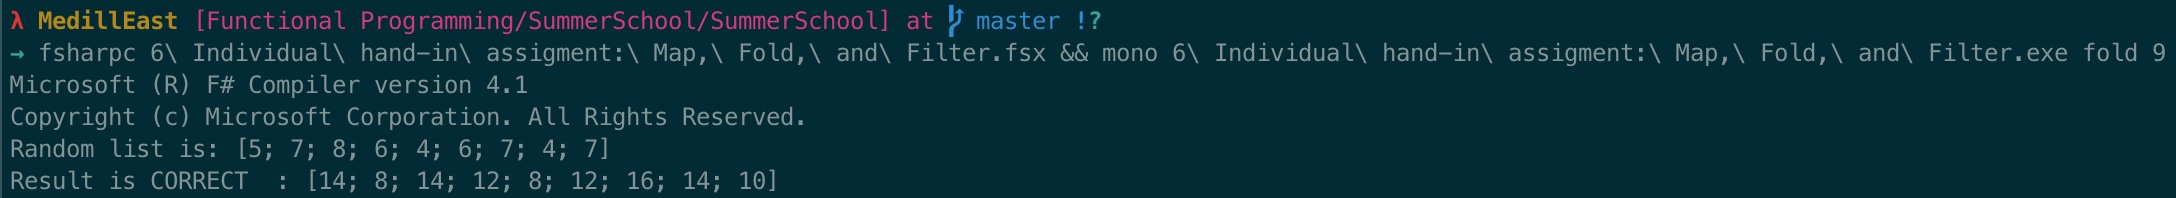
\includegraphics[width=\linewidth]{fold2}
      \caption{Testing of fold function}
      \label{fig:fold}
\end{figure}

\begin{figure}[h]
      \centering
      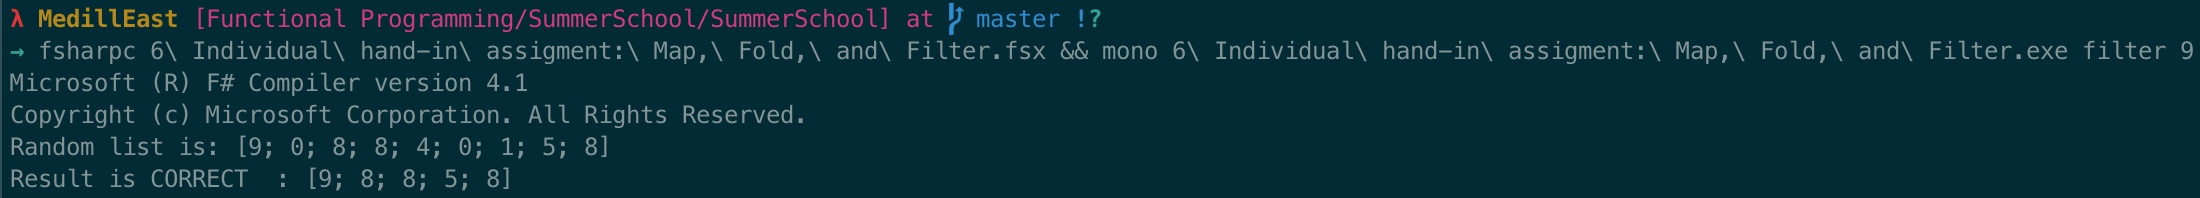
\includegraphics[width=\linewidth]{filter2}
      \caption{Testing of filter function}
      \label{fig:filter}
\end{figure}

\section{Conclusion}

In this assignment, I implemented the \emph{myFold} and \emph{myFilter} functions with my own recursive method. I stuck at the beginning of my writing, but things went smoothly when I rearranged my thoughts and wrote down the pseudocode. It's easy to get bogged down in the details of a program, but we should take a top-down functional programming approach and thinking more about what to do than how to do it.


%\renewcommand\refname{Reference\\
%\small those are reference form Week 6, I'll list Week5's reference next time}
\bibliographystyle{unsrt}
\bibliography{reference}

%\begin{thebibliography}{99}
%\bibitem{1} \href{http://research.nii.ac.jp/~takayama/metallophone/metallophone-cga2011.pdf}{Responsive FEM for Aiding Interactive Geometric Modeling} \\
%Umetani N, Takayama K. Responsive FEM for Aiding Interactive Geometric Modeling[J]. 2010.

%\bibitem{2} \href{http://www-ui.is.s.u-tokyo.ac.jp/~takeo/papers/umetani_nime2010_metallophone.pdf}{Designing Custom-made Metallophone with Concurrent Eigenanalysis}\\
%Umetani N, Mitani J, Igarashi T. Designing Custom-made Metallophone with Concurrent Eigenanalysis[J]. Data, 2010. 

%\bibitem{3} \href{http://www.jst.go.jp/erato/igarashi/publications/001/SensitiveCouture.pdf}{Sensitive Couture for Interactive Garment Modeling and Editing}\\
%Umetani N, Kaufman D M, Igarashi T, et al. Sensitive couture for interactive garment modeling and editing[C]// ACM, 2011:1-12.

%\bibitem{4} \href{http://www.jst.go.jp/erato/igarashi/en/projects/GuidedExploration/2012_siggraph_GuidedExploration.pdf}{Guided Exploration of Physically Valid Shape for Furniture Design}\\
%Umentani N, Igarashi T, Mitra N J. Guided exploration of physically valid shapes for furniture design[J]. Communications of the ACM, 2015, 58(9):116-124.

%\bibitem{5} \href{http://www.nobuyuki-umetani.com/publication/2014_sigg_pteromys/2014_siggraph_GliderDesign.pdf}{Pteromys: Interactive Design and Optimization of Free-formed Free-flight Model Airplanes}\\
%Umetani N, Koyama Y, Schmidt R, et al. Pteromys:interactive design and optimization of free-formed free-flight model airplanes[J]. Acm Transactions on Graphics, 2014, 33(4):1-10. 

%\bibitem{6} Mori Y, Igarashi T. Plushie: an interactive design system for plush toys[C]//ACM Transactions on Graphics (TOG). ACM, 2007, 26(3): 45.

%\bibitem{7} Igarashi Y, Igarashi T, Mitani J. Beady: interactive beadwork design and construction[J]. ACM Transactions on Graphics (TOG), 2012, 31(4): 49.
 
%\bibitem{8} Saul G, Lau M, Mitani J, et al. SketchChair: an all-in-one chair design system for end users[C]//Proceedings of the fifth international conference on Tangible, embedded, and embodied interaction. ACM, 2011: 73-80.
 
%\bibitem{9} Saakes D, Cambazard T, Mitani J, et al. PacCAM: material capture and interactive 2D packing for efficient material usage on CNC cutting machines[C]//Proceedings of the 26th annual ACM symposium on User interface software and technology. ACM, 2013: 441-446.

% \bibitem{10} A. Rovira, D. Swapp, B. Spanlang, and M. Slater. The use of virtual reality in the study of people’s responses to violent incidents. Frontiers in Behavioral Neuroscience, 3(59), 2009. doi: 10.3389/neuro.08.059.2009
 %\bibitem{11} J.Russell.Agency:itsroleinmentaldevelopment.EssaysinEnvironmen- tal Psychology. Psychology Press, East Sussex, UK, 1996.
 %\bibitem{12} R.Skarbez.Apreliminaryinvestigationofplaceillusionandplausibility illusion. In IEEE Virtual Reality (VR) Doctoral Consortium, 2015.
 %\bibitem{13} M.Slater.Placeillusionandplausibilitycanleadtorealisticbehaviorin immersive virtual environments. Philosophical transactions of the Royal Society of London. Series B, Biological sciences, 364:3549–3557, 2009.
 %\bibitem{14} M. Slater, P. Khanna, J. Mortensen, and I. Yu. Visual realism enhances realistic response in an immersive virtual environment. IEEE Computer Graphics and Applications, 29:76–84, 2009. doi: 10.1109/MCG.2009.55
 %\bibitem{15} M. Slater, B. Spanlang, and D. Corominas. Simulating virtual environ- ments within virtual environments as the basis for a psychophysics of presence. ACM Trans. Graph., 29:92:1–92:9, July 2010. doi: 10.1145/ 1778765.1778829
 
%\end{thebibliography}



\end{document}